\documentclass[a4paper,11pt]{article}

\usepackage{graphicx}
\usepackage{subfig,hyperref}
\newcommand{\HRule}{\rule{\linewidth}{0.5mm}}

\begin{document}
\pagenumbering{alph}
\begin{titlepage}
\begin{center}

\textsc{\LARGE CMSC726 Machine Learning}\\[1.5cm]

\textsc{\Large Project 3}\\[0.5cm]

\HRule \\[0.5cm]

{ \huge \bfseries Unsupervised Learning}\\[0.4cm]

\HRule \\[1.5cm]

{\large Angjoo Kanazawa, Ran Liu, and Austin Myers}

\vfill

{\large December 6, 2011}

\end{center}
\end{titlepage}
\pagenumbering{arabic}

\section{PCA and Kernel PCA}
\subsection{WU1}
\textsf{Depending exactly on your random data, one or more of these lines might
not pass exactly through the data as we would like it to. Why not?}\vspace{0.1in}

\subsection{WU2}
\textsf{Plot the normalized eigenvalues (include the plot in your writeup). 
How many eigenvectors do you have to include before you've accounted 
for 90\% of the variance? 95\%? (Hint: see function cumsum.)}\vspace{0.1in}

% \begin{figure}[!ht]
%   \begin{center}
%   \caption{Plot of the normalized eigenvalues}
%   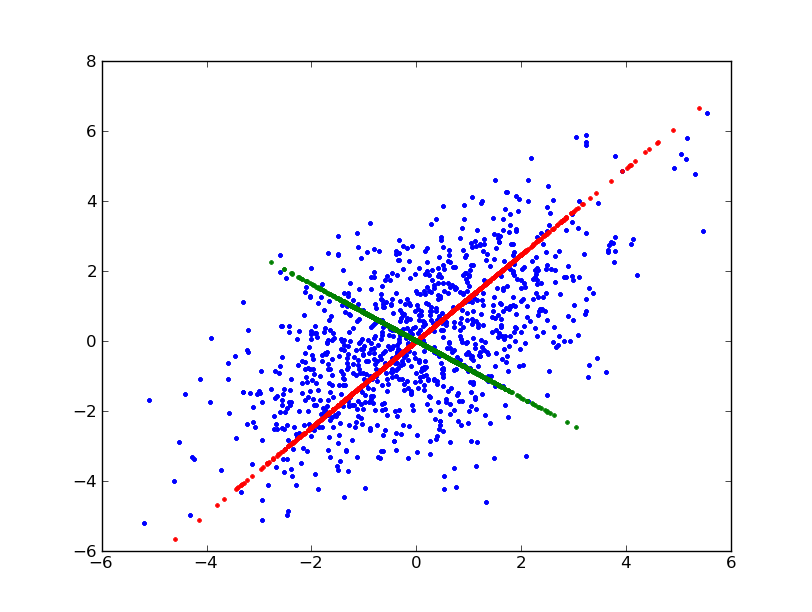
\includegraphics[width=4.5in]{pca.png}
%   \label{figures:wu61}
%   \end{center}
% \end{figure}

\subsection{WU3}
\textsf{Do these look like digits? Should they? Why or why not?
(Include the plot in your write-up.)}\vspace{0.1in}

% \begin{figure}[!ht]
%   \begin{center}
%   \caption{Plot of digits using vanilla pca}
%   \includegraphics[width=4.5in]{pca_digits.png}
%   \label{figures:wu61}
%   \end{center}
% \end{figure}

\subsection{WU4}
\textsf{Why does vanilla PCA find this data difficult? What is the
significance of the relatively large value of the eigenvalues here?}\vspace{0.1in}

\subsection{WU5}
\textsf{Did PCA do what we might want it to? Why or why not? Include
the plot to justify your answer.}\vspace{0.1in}

% \begin{figure}[!ht]
%   \begin{center}
%   \caption{Pca doing what we want..}
%   \includegraphics[width=4.5in]{pca2.png}
%   \label{figures:wu61}
%   \end{center}
% \end{figure}

\subsection{WU6}
\textsf{How do the eigenvalues here compare to the linear case? What
does this tell you? How does the plot look? How might this be useful
for supervised learning?}\vspace{0.1in}

% \begin{figure}[!ht]
%   \begin{center}
%   \caption{Using KPCA}
%   \includegraphics[width=4.5in]{pca2.png}
%   \label{figures:wu61}
%   \end{center}
% \end{figure}

\subsection{WU7}
\textsf{Experiment with different kernels, and perhaps interpolations 
of different kernels. Try to find a kernel that gets as much of the 
variance on the first two principle components as possible. Report your 
kernel and a plot of the data projected into 2d under that kernel.}\vspace{0.1in}

\pagebreak
\section{HMMs:Viterbi}
\subsection{WU8}
\textsf{Find two different observation sequences of length four that
differ only in one place, but differ in more than one place in the
guessed output.}\vspace{0.1in}

%hmm.viterbi(array([0,1,1,1]), a, b, pi) # 0 0 0 0
%hmm.viterbi(array([0,1,2,1]), a, b, pi) # 0 0 1 1

One example of this effect can be found with observation sequences
[0,1,1,1] and [0,1,2,1] which differ only in the third observed emission,
but which yield predictions of [0,0,0,0] and [0,0,1,1] respectively.
Thus, the predictions differ in two states where the observations only
differ in one.

\section{HMMs:Forward-backward}
\subsection{WU9}
\textsf{Why does EM settle in this configuration? What is it saying? 
What happens when you use three states instead of two? 
What's the resulting probability of the data? 
What about four states? What happens and why?}\vspace{0.1in}
EM settles in this configuration because it is a local minima. The
$\hat \pi = [1,0,0]$ means that we always start at state 0. We also get $P(X_t=0|X_{t-1}=0)= 0$,
i.e. when we transition we always go to a different state. All
together the results say that states alternate and that is the most
likely state sequences.

If we use three states instead of two, similar behavior happens with
$\hat \pi$. One state has a probability of 1 and rest gets 0. For 

\subsection{WU10}
\textsf{Run EM on this data using two states. 
Run it a few times until you get a final log probability at least -9250. 
(It should happen in two or three trials. This will take a few minutes to run.) 
When you do this, it will print out the resulting initial state probabilities, 
transition probabilities and emission probabilities. 
What has it learned? Include all of this output in your write-up.}\vspace{0.1in}

\end{document}
